\chapter{Wstęp}
\section{Cel}
Celem tej pracy inżynierskiej jest budowa środowiska robota mobilnego w przestrzeni wirtualnej.
Za zadanie jest stworzyć oprogramowanie modelu 3D, oraz modelu dynamiki wielokierunkowej platformy mobilnej z kołami szwedzkimi. 
Wymaga się, aby model i obsługujące go oprogramowanie było dokładną kopią prawdziwego robota, dzięki czemu zachowanie symulacji będzie jak najbardziej zbliżone do zachowania fizycznego obiektu.
Opisywana platforma będzie używana jako baza wielokierunkowa do przemieszczania dwuramiennego robota manipulującego Velma.

Należy tak opisać model, aby reagował na siły podobnie do rzeczywistej wersji i przyjmował to samo sterowanie z zewnątrz, co rzeczywisty obiekt.
To spowoduje, że możliwe będzie stworzenie jednego wspólnego programu sterującego do użycia zarówno w wirtualnej wersji, jak i fizycznej.

Testowanie oprogramowania na prawdziwym obiekcie może prowadzić do jego uszkodzeń, dlatego wpierw trzeba się upewnić o poprawności projektowanych rozwiązań na bezpiecznej kopii wirtualnej.
Rzeczywistość nie pozwala także na przeprowadzanie zaawansowanych scenariuszy środowiska testowego.
Szybciej i taniej jest stworzyć wirtualne środowisko testowe, niż fizyczne, w dodatku porażka sterowników przy symulacji nie wpływa na zniszczenie robota w rzeczywistości.
Dopiero przy osiągnięciu satysfakcjonującej jakości sterowania w symulacji wirtualnej można zastosować algorytmy sterowania do oryginalnego obiektu bez ryzyka uszkodzeń urządzenia.

Należy także móc obsługiwać czujniki, za pomocą których oprogramowanie orientuje się w przestrzeni i generuje sterowanie.
Wirtualizacja czujników polega na generowaniu danych na podstawie symulacji.
W celu przybliżenia wyjścia takiego programu do rzeczywistego urządzenia, do generowanych danych zwykle dodaje się szum, oraz błędy.

\section{Wielokierunkowa platforma mobilna}

\begin{figure}[H]
\centering
 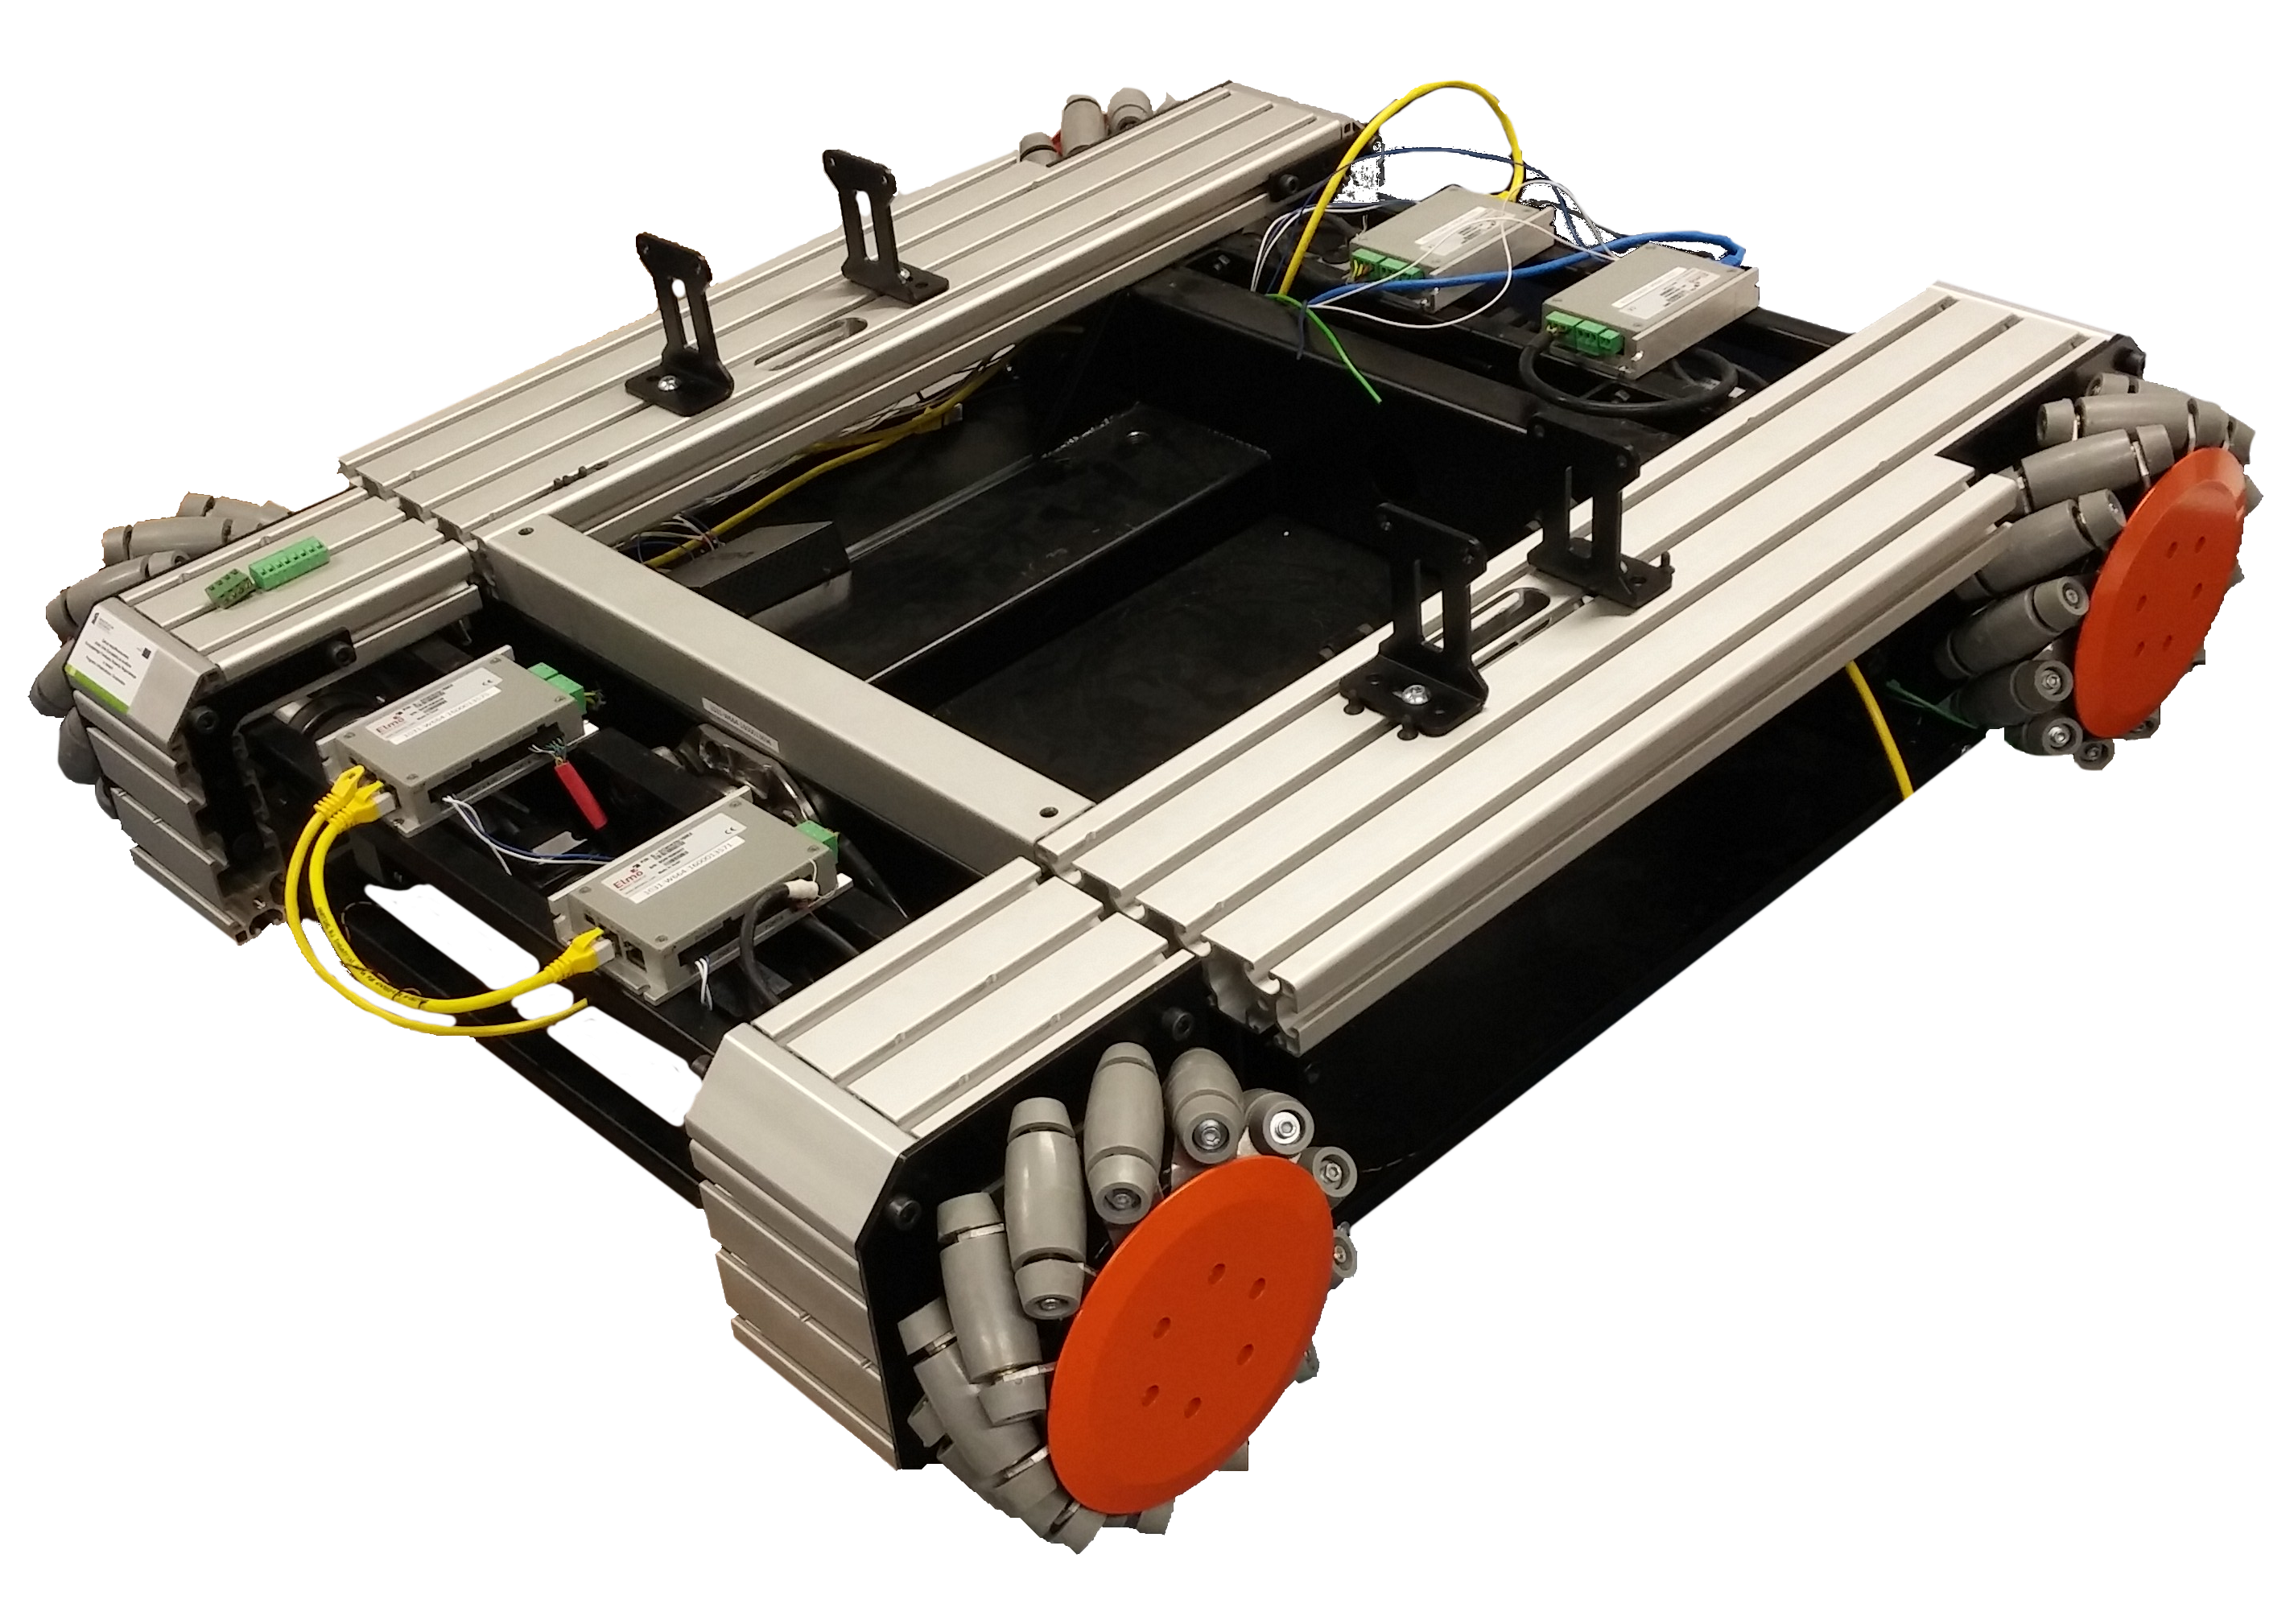
\includegraphics[width=0.8\textwidth]{graphics/base_photo.png}
\caption{Fotografia platformy z perspektywy. Niebieskie urządzenia na szczycie to czujniki laserowe. Na obecny stan koła są nieprawidłowo ustawione.}
\end{figure} 

Jest to duża, prostokątna baza dookólna poruszająca się na czterech kołach szwedzkich.
Koła są stałe, parami przyczepione do dwóch osi.
Każde koło jest sterowane osobno przez podłączony bezpośrednio serwomotor, zatem może mieć prędkość i kierunek niezależny od pozostałych kół i kierunku poruszania się robota, oraz jego obrotu.
Każdy z serwomotorów ma także wbudowany enkoder umożliwiający pomiar rzeczywistego kąta obrotu koła.

Koła szwedzkie, zwane także kołami mecanum, to specjalne koła z dodatkowymi rolkami na obwodzie ustawionymi pod kątem $45^\circ$ do osi koła.
Rolki są pasywne i obracają się niezależnie od siebie. Każde koło posiada 12 takich rolek.
Ich osie ustawione są w ten sposób, że osie rolek dwóch kół z tej samej strony robota przecinają się pod kątem prostym.
Innymi słowy, robot ma identycznie ustawione koła na przeciwległych wierzchołkach, i razem ustawione są w kształt litery \emph{X} patrząc na nie z góry.
Na obecny stan robot i jego trójwymiarowe modele mają nieprawidłowo ustawione koła.

\begin{figure}[H]
\centering
 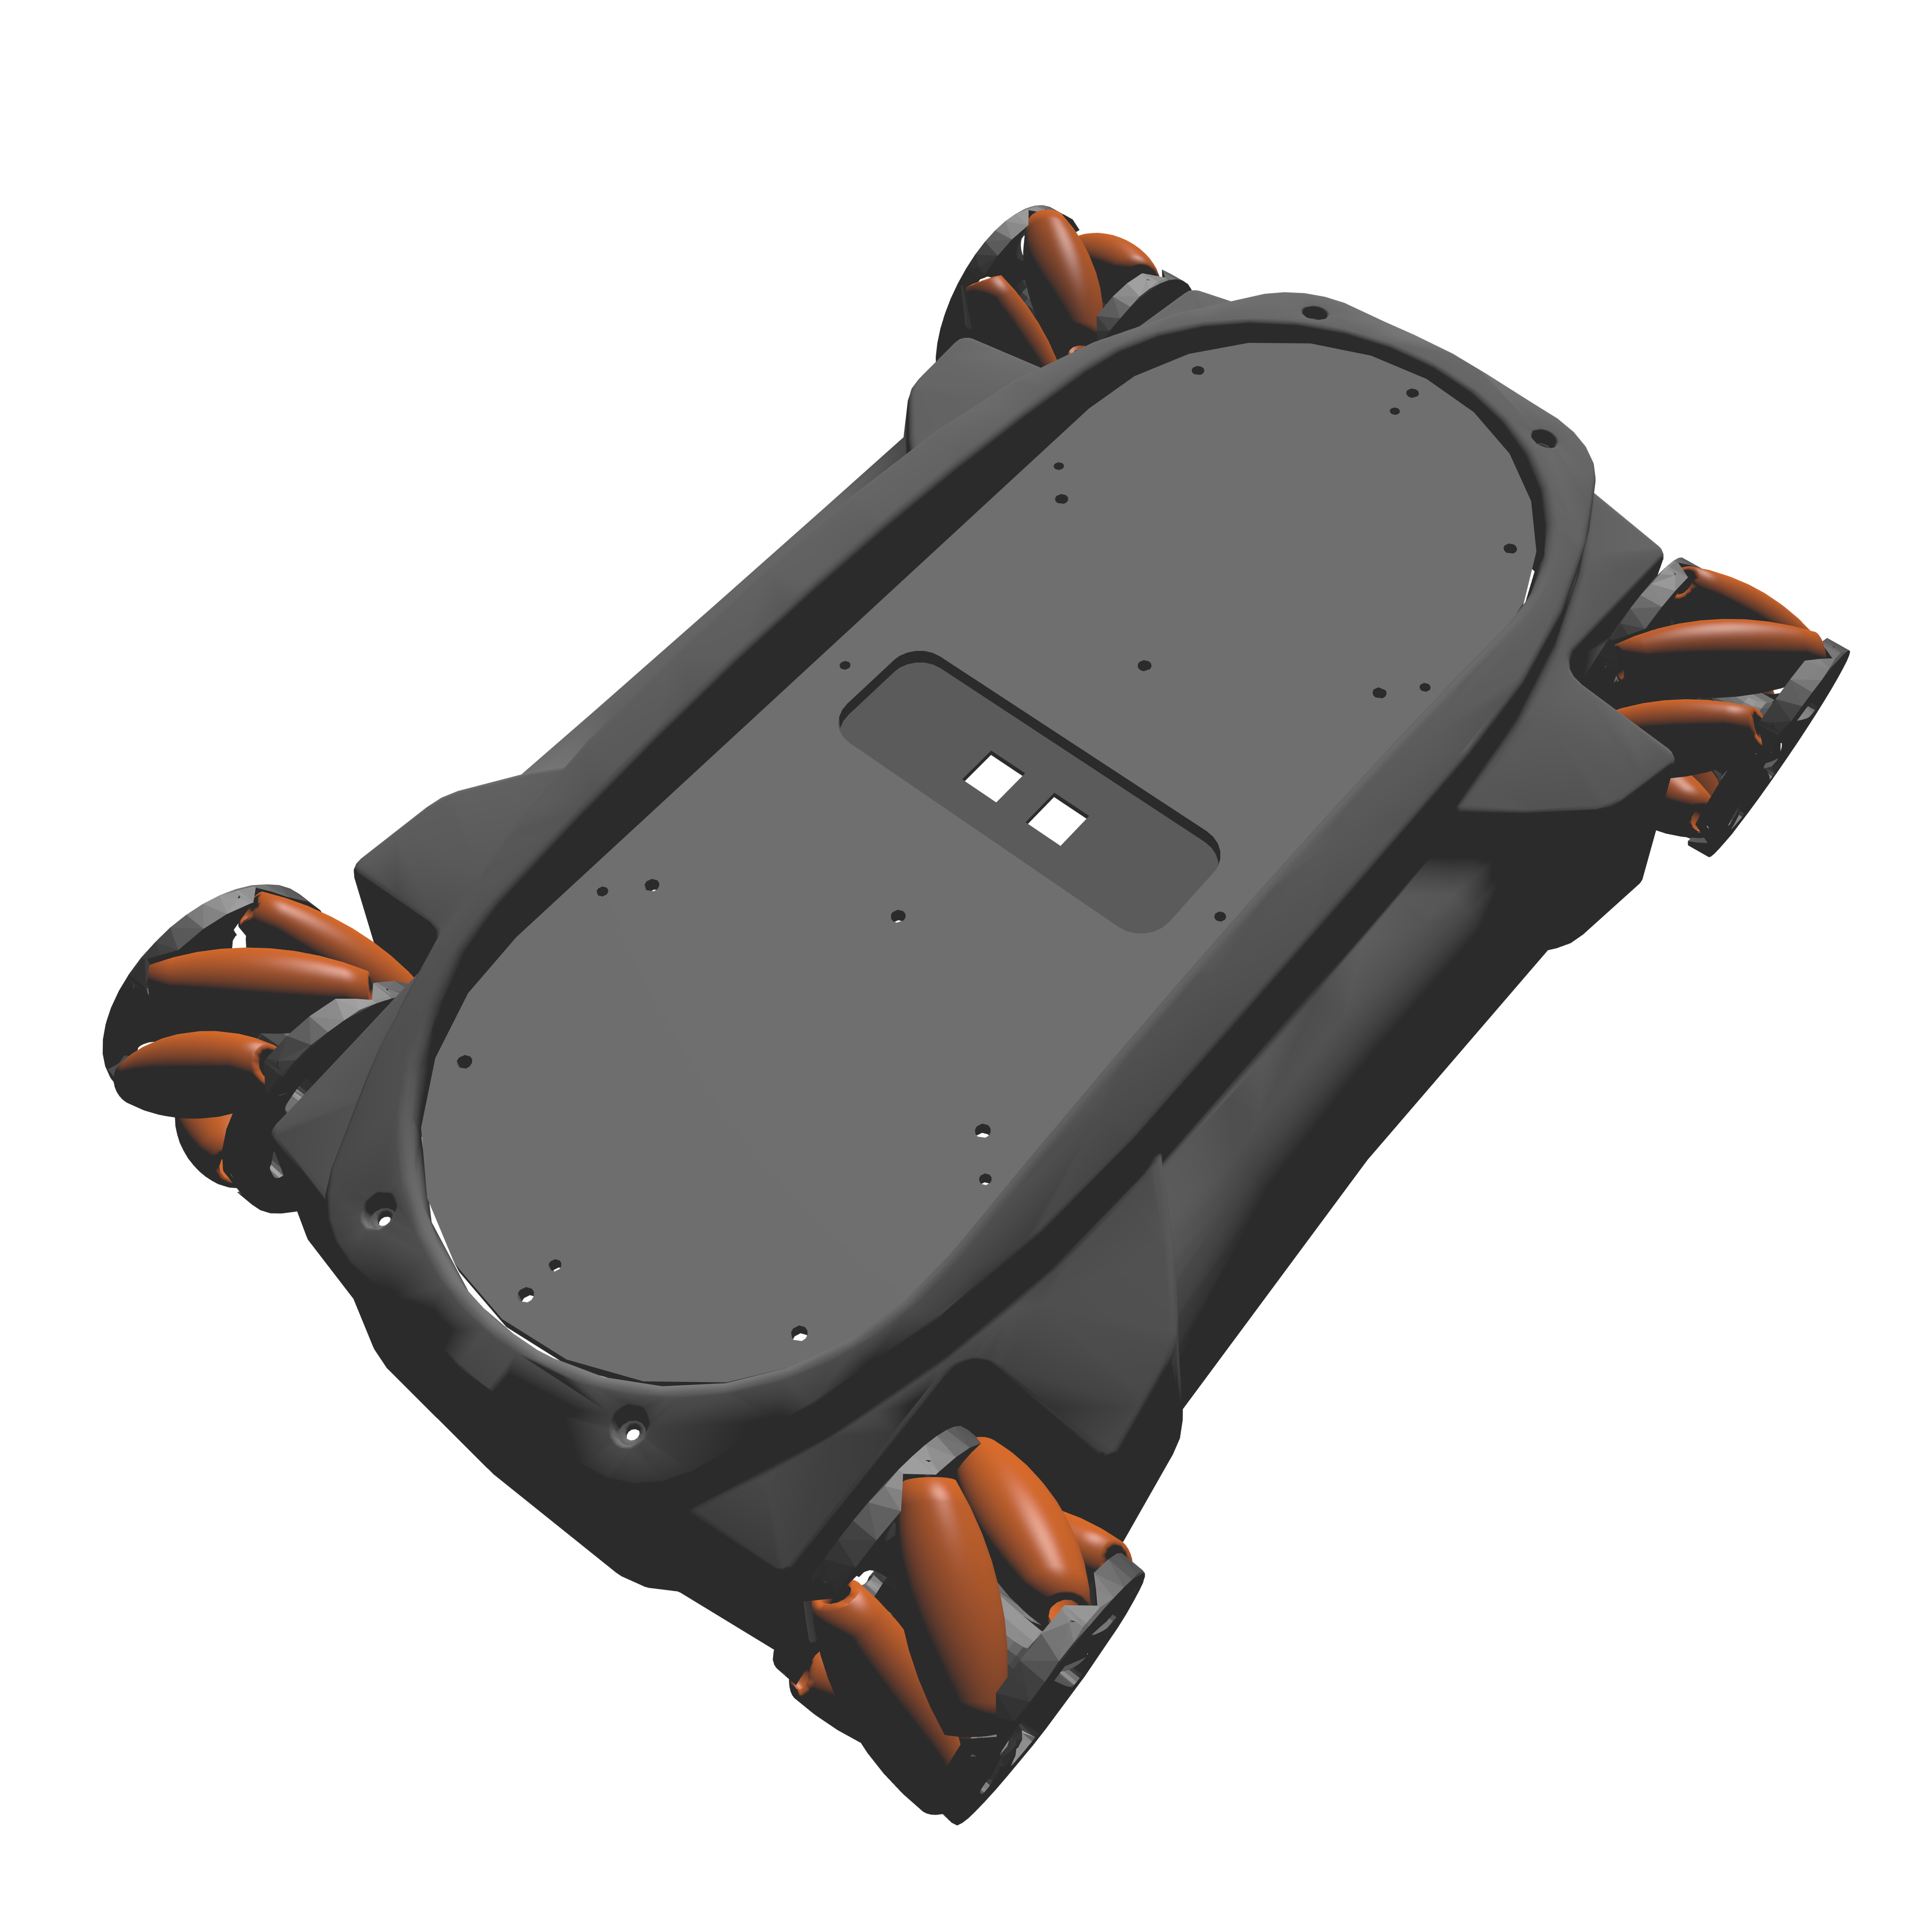
\includegraphics[width=0.8\textwidth]{graphics/kuka_youbot.png}
\caption{Przykład prawidłowej platformy wielokierunkowej na podstawie fragmentu komercyjnego robota Kuka Youbot. Należy zwrócić uwagę na charakterystyczne ustawienie kół względem siebie.}
\end{figure} 

Odpowiedni obrót kół względem bazy pozwala na jej ruch w dowolnym kierunku niezależnie od kąta obrotu robota.
Za ich pomocą da się także obracać bazą stojąc w miejscu, lub w trakcie ruchu po prostej.
Na przykład, jeśli obracać tylko przeciwległymi kołami po przekątnej, system zacznie się poruszać po skosie bez zmiany kąta obrotu.
A jeśli do tego dodamy obrót kół drugiej przekątnej w odwrotnym kierunku, wtedy pojazd zacznie się poruszać w bok pomimo faktu, że koła nie są skrętne i nie mogą ustawić się prosto do kierunku jazdy.

\begin{figure}[H]
\centering
 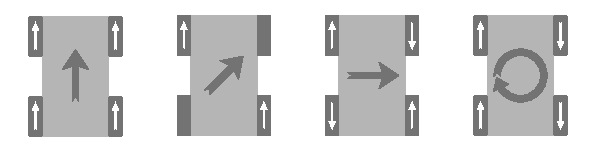
\includegraphics[width=0.8\textwidth]{graphics/mecanum_dirs.pdf}
\caption{Podstawowe ruchy, jakie może wykonywać robot o napędzie wielokierunkowym.}
\end{figure} 

Podstawa ma za zadanie transportować wydziałowego robota manipulującego Velma tworząc razem uniwersalny manipulator mobilny.
Velma to wysoki i bardzo ciężki robot wyposażony w dwa chwytaki na ramionach o licznych przegubach.
Taka budowa wymaga szerokiej podstawy, aby zachować środek ciężkości całości odpowiednio nisko.
Jeżdżąc na tej podstawie robot może się przemieszczać i obracać w dowolnym kierunku, aby uzyskać lepszy dostęp do manipulowanych przedmiotów.
Dodatkowe czujniki laserowe umieszczone tuż nad postawą odpowiadają za wykrywanie kolizji.

Platforma jest niesymetrycznie podzielona w poprzek na dwie niezależne części.
Przegub o jednym stopniu swobody (tzw. zawias) jest jedynym łącznikiem pomiędzy tymi dwoma fragmentami.
Zadaniem tego przegubu jest niwelować niedoskonałości terenu, aby każde koło dociskało do podłoża z taką samą siłą, jak po drugiej stronie osi.
Bez tego zawiasu nierówny teren uniemożliwiałby sprawne sterowanie platformą na skutek nierównego tarcia kół tej samej osi i nieplanowany skręt.
Niedeterministyczne tarcie kół jest niewykrywalne w bezpośredni sposób, więc należy je wyeliminować na przykład za pomocą takiego przegubu.

\begin{figure}[H]
\centering
 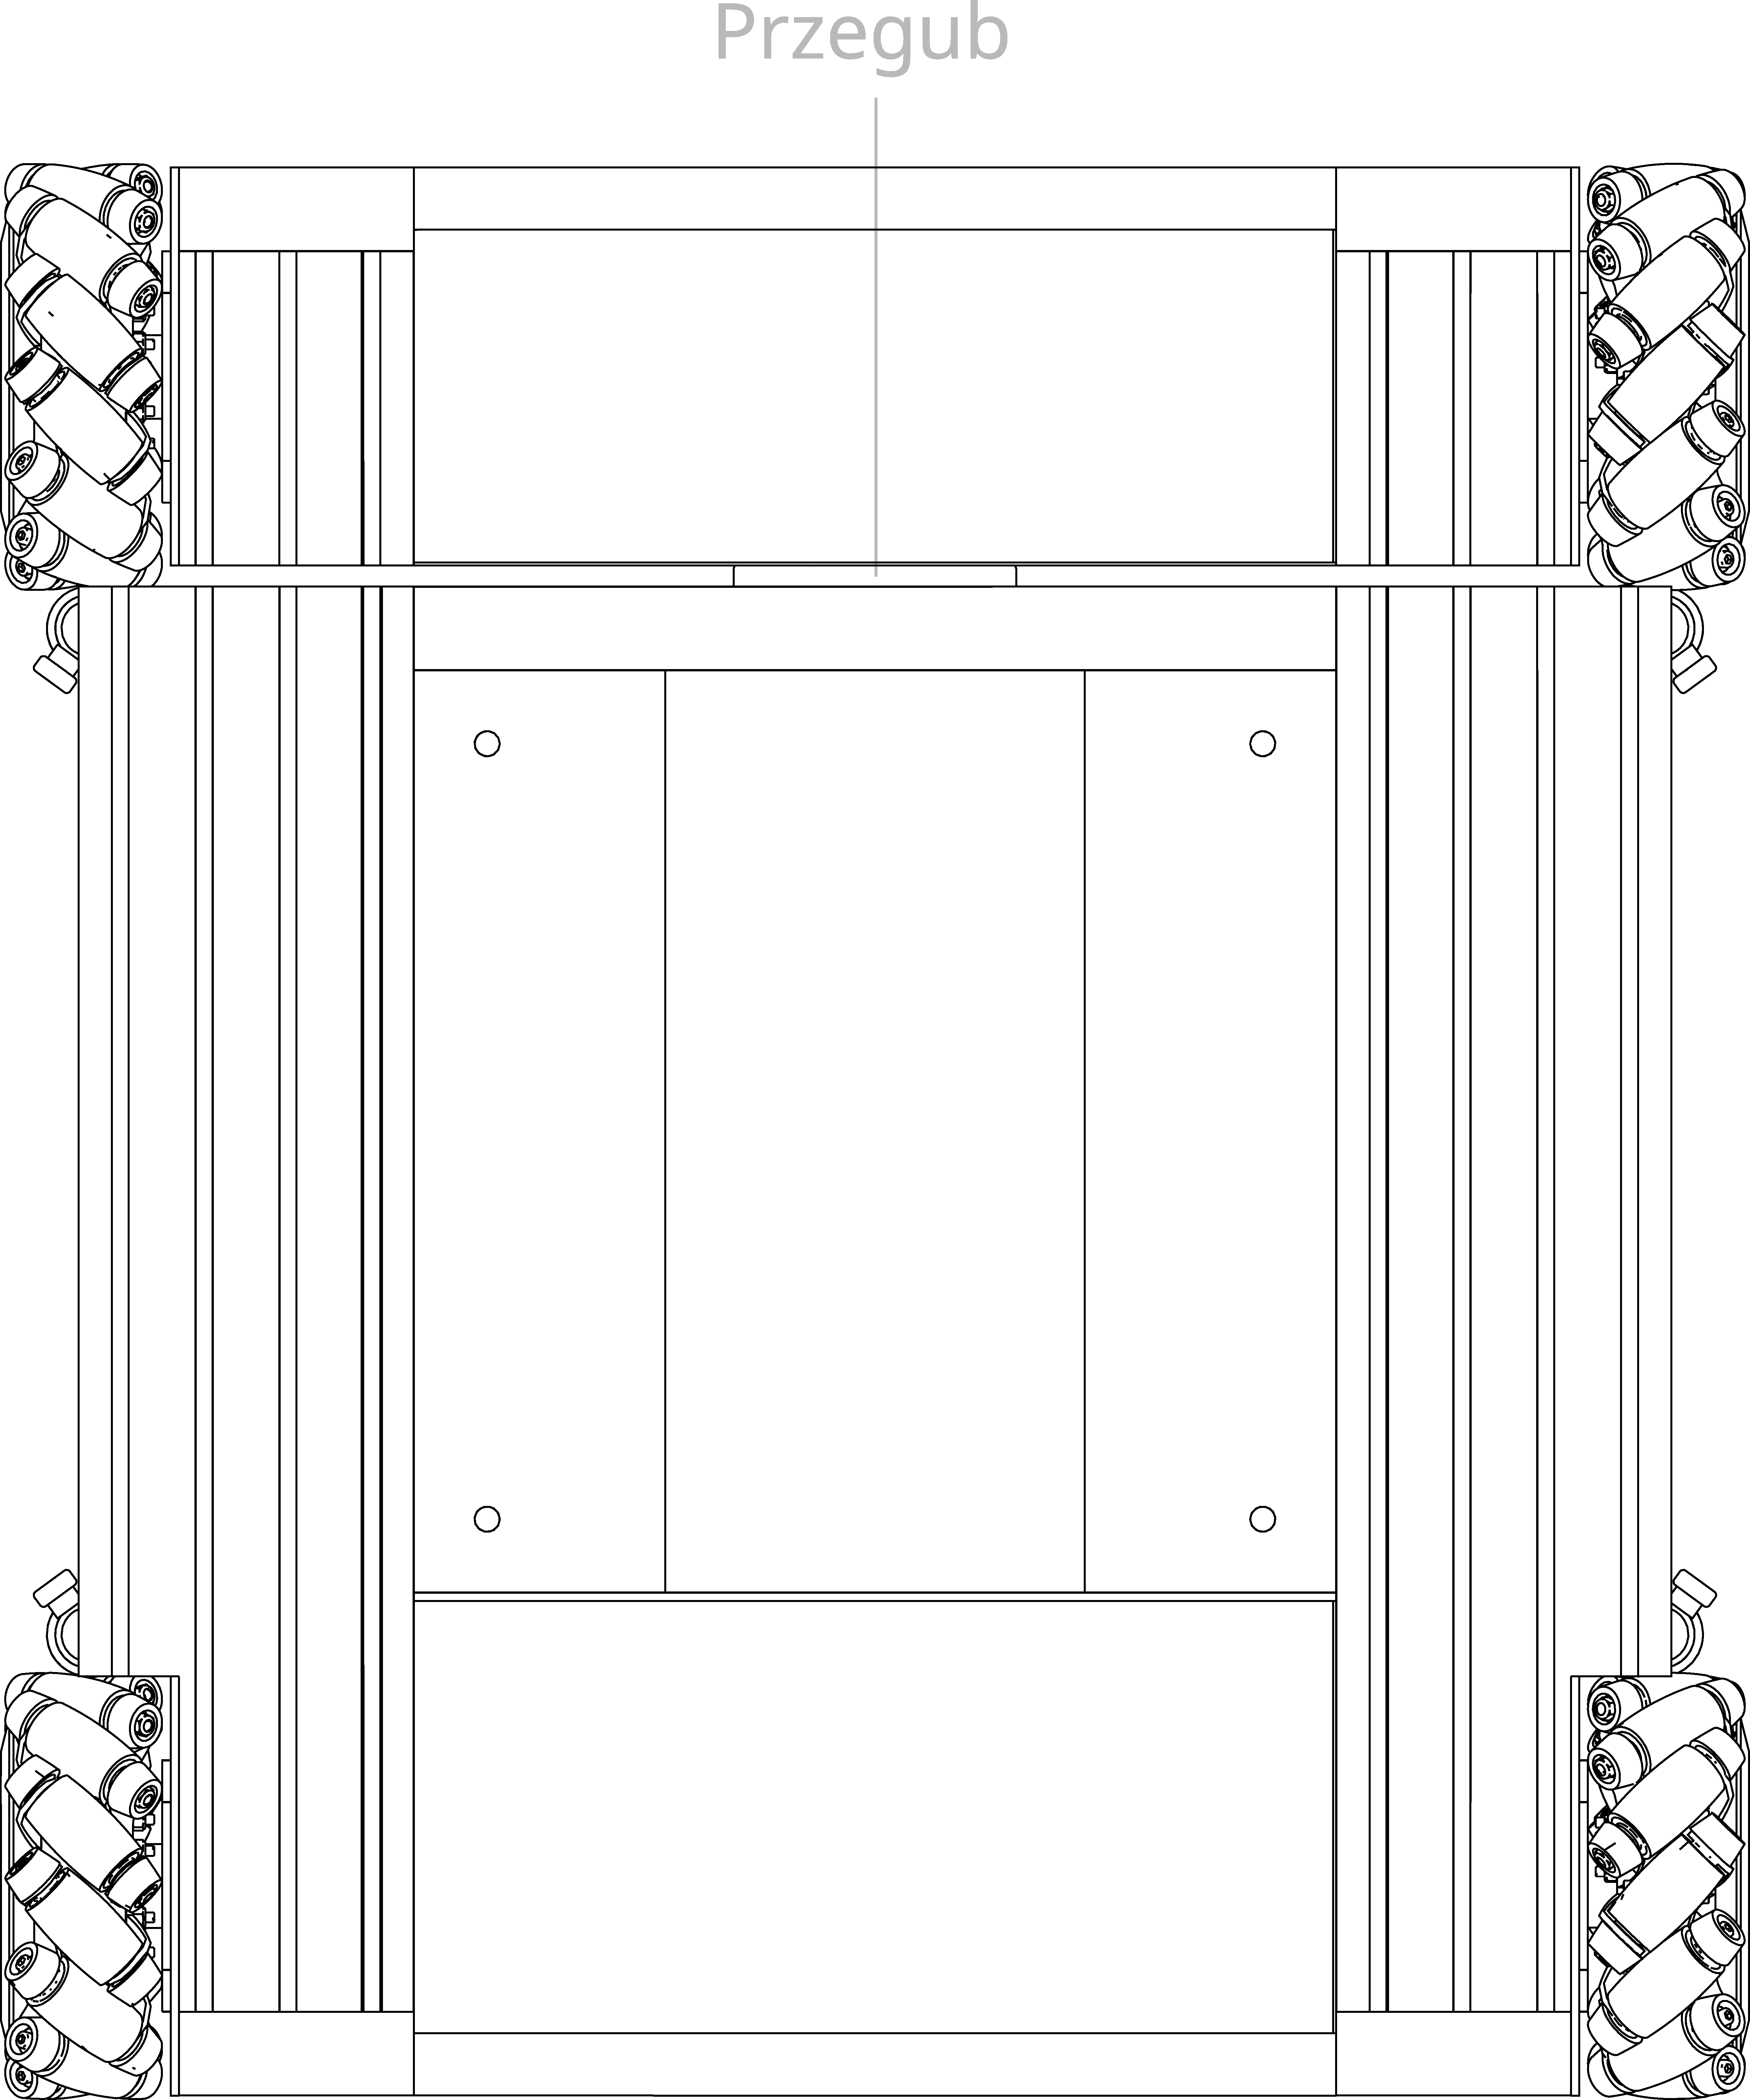
\includegraphics[width=0.5\textwidth]{graphics/base_top.pdf}
\caption{Platforma mobilna widziana od góry. Przegub zawiasowy łączy dwie części.}
\end{figure} 

\begin{figure}[H]
\centering
 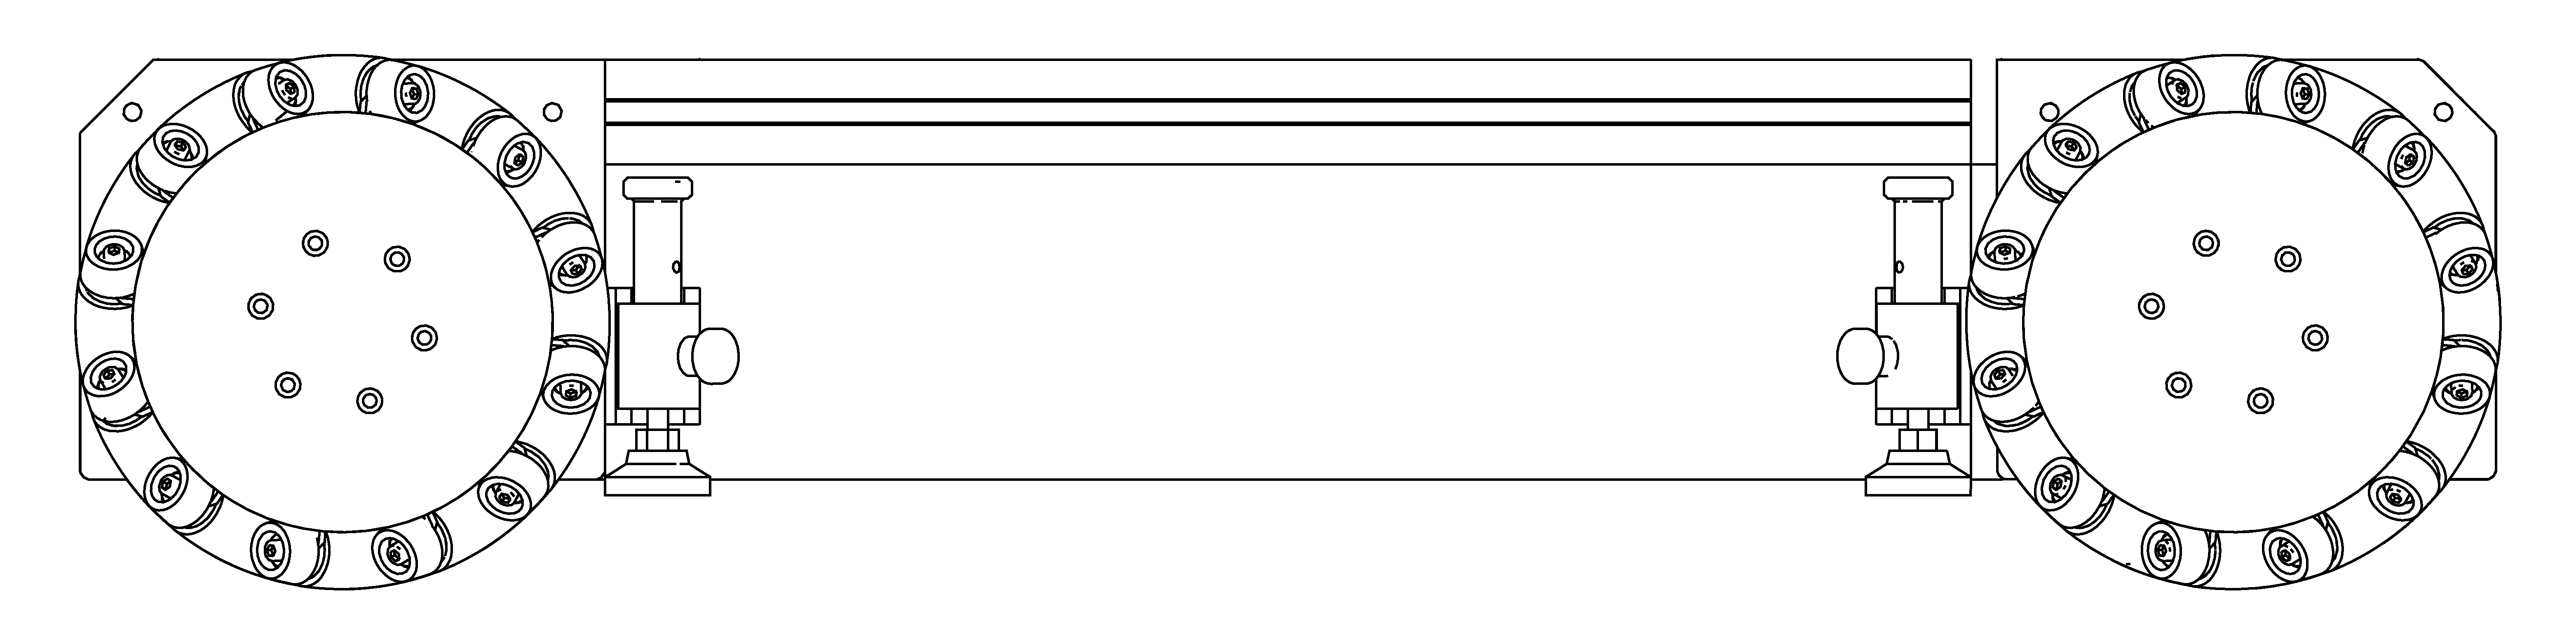
\includegraphics[width=0.5\textwidth]{graphics/base_side.pdf}
\caption{Platforma mobilna widziana od prawej strony.}
\end{figure} 

\begin{figure}[H]
\centering
 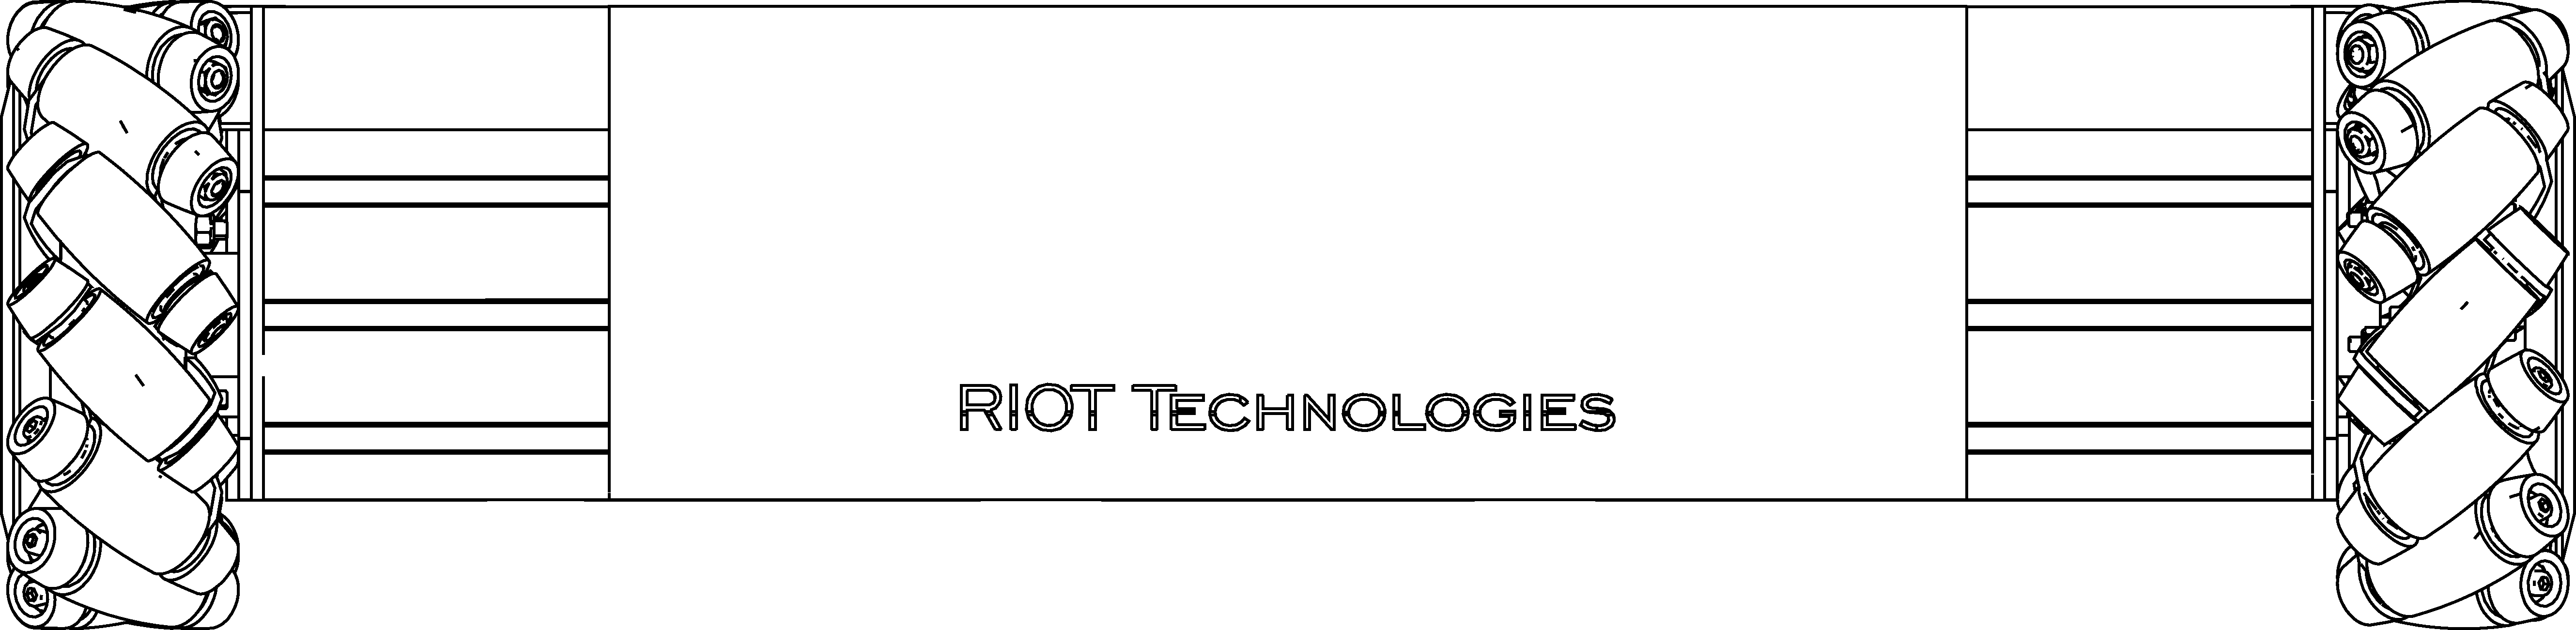
\includegraphics[width=0.5\textwidth]{graphics/base_front.pdf}
\caption{Platforma mobilna widziana od tyłu.}
\end{figure} 



\section{Składniki systemu}
Środowisko symulacyjne składa się z kilku odrębnych modułów, które komunikują się ze sobą poprzez specjalne interfejsy wykorzystujące kolejki wiadomości.
Taka implementacja komunikacji pozwala zamieniać i przepisywać kod źródłowy elementów, używać różnych języków programowania zachowując tę samą komunikację między składnikami i nie tracąc kompatybilności między sobą.

Efektor rzeczywisty, na przykład serwomotor jest sterowany za pomocą efektora wirtualnego, który zamienia wyjście głównego układu sterowania na zrozumiałe dla silnika wartości fizyczne. 
Przykładowo zmienia podaną liczbę oznaczającą zadaną prędkość na odpowiednie napięcie na wyjściu. W przestrzeni symulacyjnej jedynie wywołuje odpowiednie funkcje maszyny do symulacji.

Podobnie receptor wirtualny pobiera surowe dane z czujnika, przekształca na odpowiedni format, usuwa błędy i szum tak, aby program sterujący mógł wykorzystać te dane w prosty sposób. 
Doskonałym przykładem jest tutaj kamera Kinect, w której to zachodzi odczytanie obrazu z kilku kamer i zamiana na mapę odległości, szkielety wykrytych osób, ich sylwetki i wiele innych gotowych danych.

%TODO Zmienić na Tikz
\begin{figure}[H]
\centering
 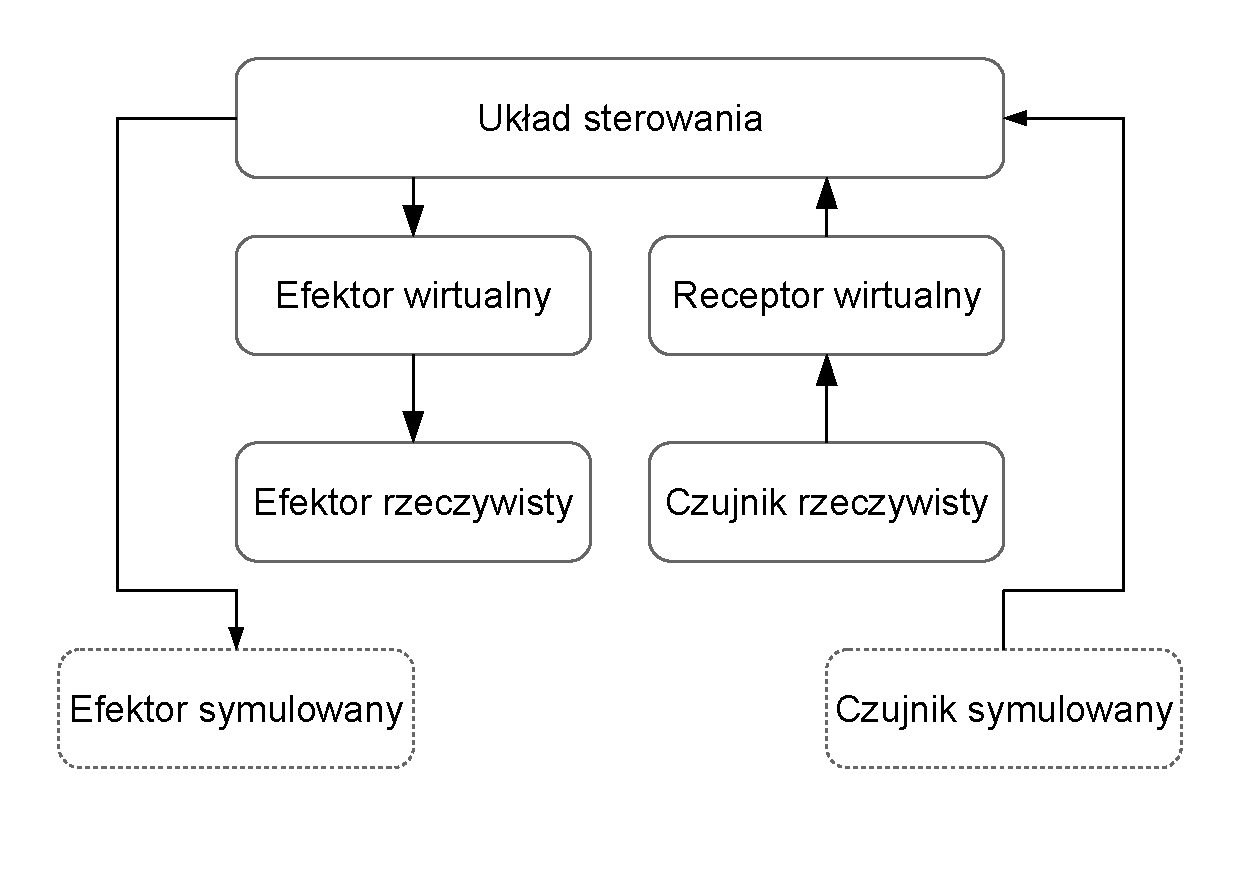
\includegraphics[width=0.5\textwidth]{graphics/agent.pdf}
\caption{Struktura agenta upostaciowionego.}
\end{figure} 


\subsection{Model 3D}
 Odpowiednio opisany równaniami fizycznymi powinien mieć zachowanie zbliżone do oryginału w jak największym stopniu.
 Musi brać pod uwagę masy i momenty bezwładności elementów składowych, a także wszelkie tarcia.
 Model posiada więzy na ruchome elementy, jak koła i rolki, aby symulować przeguby.
 
 Ta część środowiska oddziałuje bezpośrednio z maszyną do symulacji fizycznej. 
 To kształt, masy i momenty bezwładności brył są argumentami funkcji liczących.
 Także maszyna manipuluje z powrotem podanymi obiektami nadając im wirtualnie odpowiednie prędkości w czasie.
 
 Do modelu doczepia się wirtualne czujniki generujące odpowiednie dane na podstawie symulacji i rozkładu losowego.
 Nie są to pełne dane o stanie modelu, jakie posiada maszyna do symulacji, gdyż czujniki fizyczne również nigdy nie mają pełnej informacji o stanie urządzenia.
 
 Dla ozdoby można wykorzystać istniejący model CAD do stworzenia siatki trójwymiarowej i nadania symulowanemu obiektowi wyglądu zbliżonego do fizycznego robota.

 \subsection{Sterownik silników}
Program sterujący generuje abstrakcyjne dane, na przykład liczbę zapisaną binarnie.
Przykładowy silnik fizyczny nie jest w stanie działać na ich podstawie, on potrzebuje odpowiedniego napięcia na wejściu.
Do tłumaczenia jednych danych na drugie potrzebny jest sterownik niskopoziomowy.
Najczęściej implementowany jest w formie mikrokontrolera, lub podobnego systemu wbudowanego.

Jego zadanie to odczytanie danych podanych przez program sterujący i na przykład generowanie na ich podstawie odpowiedniej fali PWC, lub obsługa przetwornika cyfrowo-analogowego.
Do innych zadań może należeć kontrola, czy żądana wartość nie uszkodzi urządzenia.
Zazwyczaj sterownik może komunikować się z powrotem z resztą systemu, aby zgłaszać ewentualne awarie.

Taki program i powiązany z nim układ elektroniczny są najczęściej dostarczone przez producenta robota i są nieznany użytkownikowi.
Dodatkowo tworzy kolejną warstwę abstrakcyjną dla sterownika głównego, który nie musi zważać na generowanie różnych danych dla różnych typów efektorów.
 
W środowisku wirtualnym należy stworzyć moduł o podobnym działaniu.
Powinien przyjmować dane w dokładnie takim samym formacie, jak opisany wyżej układ, aby był łatwo wymienialny na sterownik fizycznego urządzenia bez ingerencji w główny program sterujący.
Zamiast zamieniać odczytane dane na analogowe wartości, on wywołuje odpowiednie funkcje maszyny symulacyjnej, aby wywołać taki sam efekt, co na rzeczywistym efektorze, lecz w wirtualnej przestrzeni symulacji.
Jako argumenty podaje parametry fizyczne symulowanego obiektu, oraz przyłożone siły.
 

\subsection{Sterownik czujników}
Implementowany podobnie do sterownika silników ma za zadanie konwertować surowe i obarczone błędami dane z czujników na format zrozumiały dla programu sterującego.
W tym miejscu usuwa się błędy grube, niweluje stałe na podstawie kalibracji, wygładza szum i interpretuje dane, aby pozyskać wymagane przez wyższe warstwy informacje.

Przykładowo czujniki laserowe zwracają jedynie ciąg pomiarów, ale to do tego programu należy interpretacja wykrytych kształtów, łączenie punktów i obróbka do formatu zrozumiałego dla wyższych podzespołów.
Większość zaawansowanych receptorów posiada owe układy cyfrowe i programy, są wbudowane w urządzenie.
Dostarczone przez producenta tak samo, jak sterowniki efektorów.
 
Symulując ten element budujemy program generujący dane na podstawie aktualnego stanu maszyny do symulacji w sposób, w jaki działa czujnik w rzeczywistości.
Na przykład dla czujnika laserowego wypuszczamy setki promieni i obliczamy ich punkty przecięcia się z wirtualnymi modelami.
Możemy renderować obraz, aby symulować kamerę.

Ponieważ dane fizyczne nigdy nie są idealne, w celu przybliżenia wyjścia wirtualnego czujnika do oryginału, dodajemy szum o odpowiednim rozkładzie i błędy.

\subsection{Program sterujący}
Cześć odpowiedzialna za logikę aplikacji. Tutaj obliczane jest sterowanie na podstawie dostarczonych odczytów z czujników.
Zazwyczaj wykorzystuje się tu dużą ilość bibliotek dostarczających zaawansowane algorytmy.
Ich zadania mogą polegać na budowie wewnętrznej mapy, wyznaczaniu ścieżki, omijaniu przeszkód, odwrotnej kinematyce i tym podobnych.

Taki program zwykle działa na mocniejszych układach, niż sterowniki ze względu na duże zapotrzebowania na moc obliczeniową.
Jeśli robot komunikuje się z użytkownikiem, lub zwraca dane, to zachodzi to w tym module. 

Programy sterujące mogą być implementowane w językach wysokopoziomowych, nawet skryptowych, gdyż wymagania czasowe nie są rygorystyczne.
Co więcej, często się zdarza, że odpowiednie składowe programu bazują na różnych technologiach.

Środowisko symulacyjne powinno zapewnić pełną abstrakcję komunikacji tego modułu.
Oznacza to, że nie zależnie, czy program działa na rzeczywistym robocie, czy symulacji wirtualnej, zawsze powinien móc komunikować się i otrzymywać dane w tym samym formacie.
W idealnym świecie program nie powinien mieć możliwości stwierdzić, czy steruje symulacją, czy oryginałem.

\section{Technologie}
Symulator daje użytkownikowi do dyspozycji odpowiedni silnik fizyczny w którym odbywa się symulacja modelu, oraz API do obsługi.
Zaawansowany silnik powinien obsługiwać odpowiednie tarcia, więzy, siły, materiały fizyczne i wszystko, co potrzebne do jak najwierniejszego odtworzenia prawdziwego zachowania obiektu.
Na rynku jest wiele różnych silników zarówno do symulacji w czasie rzeczywistym, jak i do wyznaczania tras obiektów po długich obliczeniach.
Jedne z technologii są otwartoźródłowe, inne mniej.

\subsection{Gazebo}
Ten silnik jest dość prosty w obsłudze i wydaje się mieć mało funkcji ze względu na prosty interfejs.
Jednak jego potencjał tkwi w argumentach linii poleceń i w czytaniu podanych plików.

Program symuluje podane obiekty używając jednego z czterech popularnych silników fizycznych: ODE, Bullet, Simbody lub DART.
Wszystkie te silniki są wolnym oprogramowaniem i używane także w innych programach, jak na przykład Blender.

Program oprócz symulatora ma wbudowany edytor modeli i budynków w którym możemy tworzyć nasze dzieła od razu w przestrzeni trójwymiarowej.
Jakość wykonania tych składników jest bardzo słaba, brak jest tak podstawowych funkcjonalności, jak cofanie ruchu.
Również tworząc modele w ten sposób nie mamy nad nimi pełnej kontroli i dokładności.

Zatem najlepszym sposobem jest tworzenie modelu w specjalnym formacie SDF. Jest to ustandaryzowany zdefiniowany zewnętrznie format do opisywania składników robotów i czujników.
Dzięki temu napisany w ten sposób model może być użyty także gdzie indziej, pod warunkiem przestrzegania standardu.
Składnia jest zwykłym plikiem XML, co znaczy, że może być tworzony na każdym edytorze tekstowym.

Wtyczka do sterowania modelem jest zwyczajną biblioteką dołączaną w czasie symulacji. 
Pisze się ją w C++ jako własna klasa dziedzicząca po klasie wtyczki Gazebo.
Dodatkowo tym sposobem może się łączyć z programem sterującym poprzez kolejki wiadomości udostępnione przez Gazebo, lub inne mechanizmy, nawet systemowe, jak gniazda, czy pamięć współdzielona.

Program działa domyślnie na dystrybucji Ubuntu, ale bez problemu można go także skompilować pod inne systemy.
Interfejs jest dopracowany i przestrzega wielu ustawień systemowych, jak DPI.
Uruchamianie jest proste i nie wymaga dodatkowych ustawień, tworzenia odpowiednich katalogów, czy definiowania zmiennych systemowych.
Podobnie do wszystkich tworzy ukryty katalog w katalogu domowym użytkownika, gdzie znajdują się wszystkie modele i logi.

\subsection{V-Rep}
Duży i skomplikowany silnik reklamujący się wieloma zaawansowanymi mechanizmami.
Bogaty interfejs graficzny zakłada budowę i symulację wszystkiego w tym jednym programie.

Używa dwóch z silników z Gazebo, czyli ODE i Bullet, oraz Vortex i Newton. Z tej czwórki tylko Vortex ma zamknięty kod.
Podobno symulacja fizyczna jest gorszej jakości, niż w Gazebo.

Problemem jest także zapisywanie utworzonych w programie modeli.
Program zapisuje drzewiastą strukturę modelu w pliku binarnym własnego formatu, co uniemożliwia edycję i oglądanie modelu bez posiadania całego programu i wczytywania pliku.
Brak przenośności, czy wsparcia kontroli wersji dla takich zbiorów bajtów także jest problemem.

Pisanie wtyczek najczęściej odbywa się w C. Są też dostępne inne języki skryptowe, jak Lua, Matlab, Java itp.
Komunikacja z innymi programami odbywa się poprzez specjalne mosty w formie dodatków.
API pozwala nam stworzyć mały interfejs graficzny do sterownia symulacją poprzez przyciski i suwaki.

Ze strony producenta pobieramy gotowe archiwum z programem, który nie wymaga żadnej instalacji i posiada wszystkie potrzebne zasoby do pracy i nauki, jak przykładowe modele istniejących komercyjnych robotów.
Program działa na trzech Najpopularniejszych systemach operacyjnych --- Windows, Linux i OS X.

Lepiej jednak jest używać do symulacji Gazebo głównie ze względu na jego otwartość, prostotę i elastyczność.

\subsection{ROS}
Najpopularniejsza biblioteka i gotowe algorytmy do budowania logiki sterowania.
Dostępne są tutaj programy do obróbki danych, wyznaczania ścieżek, tworzenia map itp.

Właściwie nie ma dobrej alternatywy do zbioru tych bibliotek, poza implementacją wszystkiego ręcznie na nowo i po swojemu.
Programy dla ROS pisze się w C++ i integruje z robotem za pomocą kilku gotowych struktur.

Instalacja programu na komputerze jest dużym problemem.
Z wyjątkiem Ubuntu nie ma łatwego sposobu na wgranie go do innych systemów.
Na przeszkodzie stoją błędy kompilacji dla nowszych wersji kompilatorów i inne problemy wykonania, jak naruszenie ochrony pamięci. 
Niektórym studentom wydziału się udało tego z wielkim trudem dokonać, lecz dużo prościej jest użyć Ubuntu na maszynie wirtualnej, bądź dysku USB.
Takie rozwiązanie także daje dostęp do najnowszej wersji \emph{Kinetic Kame} niedostępnej jeszcze na innych dystrybucjach.

Uruchomienie systemu wymaga wielu dodatkowych komend inicjalizujących, a także dopisywania wielu plików konfiguracyjnych za pomocą wielu skryptów do tworzonych projektów.
Używanie linii poleceń wymaga ustawienia kilku zmiennych systemowych.
Użycie niektórych funkcji wymaga uruchomionego demona serwera w tle.
Ogólnie instalacja i używanie ROS na systemie dużo śmieci, dlatego lepiej jest trzymać ją z dala od codziennego systemu operacyjnego na maszynie wirtualnej, lub dysku.

\section{Ogólny zarys pracy}
\begin{enumerate}
 \item Należy stworzyć model w SDF zachowując wszystkie rozmiary i momenty prawdziwego robota.
Należy ustawić bryły, aby przypominały kształtem podstawę i nadać im parametry fizyki.

\item Trzeba zdefiniować wszystkie więzy na koła i przegub i zamodelować je, aby silnik fizyczny dobrze współpracował.
Taki model powinien na tym stanie reagować na zewnętrzne siły, ale nie ruszać się własnymi silnikami.
Można go prosto przetestować działając siłą na elementy i patrząc, czy reaguje w poprawny sposób.

\item Wtyczka sterująca w Gazebo odczytuje dane z zewnątrz i odpowiednio obraca kołami.
Na tym poziomie można dobudować zamiennik programu sterującego jedynie do podawania prostego sterowania na koła, bez żadnej logiki.
Do komunikacji użyć struktur Gazebo, a nie ROS.
Model powinien poprawnie reagować na proste wejście, jak naprzemienne koła itp.

\item Wtyczki dla czujników, aby generowały dane z enkoderów, oraz ewentualnie innych urządzeń, dodawały błędy pomiarowe i wysyłały je na zewnątrz, aby program sterujący miał dane do działania.
Taki model jest w tym momencie kopią prawdziwego robota.

\item Program sterujący w ROS. Największy i najbardziej skomplikowany element, na szczęście wspólny dla obu bytów --- wirtualnego i rzeczywistego.
Zazwyczaj nie jest to praca jednego człowieka, a jego rozwój nie ustaje przez długi czas.
Ten program dostarczy funkcji ruchów wywoływanych przez wyższy sterownik Velmy.

\end{enumerate}

\section{Pomocne implementacje}
Istnieją już wcześniejsze modele jeżdżących robotów na kołach szwedzkich.
Można z nich brać przykład i sugerować się źródłami kodu i modelów.

Kuka Youbot jest popularnym robotem tego typu. Jego modele są domyślnie dostępne zarówno w Gazebo, jak i w V-Rep.
Tylko w przypadku V-Rep mamy wstępny sterownik do którego kierujemy zadane prędkości kół za pomocą graficznego interfejsu.
Wersja dla Gazebo symuluje kłodę drewna.

Te profesjonalne modele także pomogą przy wstępnej weryfikacji zachowania się naszego modelu, czy nie zachowuje się nadzwyczaj dziwnie.
